The \gls{galapagos} architecture is a \gls{MIMD} architecture with shared memory.
In the \Gls{barricelli} computer, a central memory controller is responsible for synchronizing memory access on the shared data bus.
Each component that wants to access memory must go through the memory controller, and follow the proper memory access request protocol.
The controller is constructed in a way that only allows one fitness core to be able to carry out a memory request at a single time.
In case of multiple memory requests, the controller performs a selection deciding in which order the requesting cores is granted the bus.
The precise technique of selection can be seen in algorithm \ref{algorithm:round-robin-selection}.
This may introduce a potential bottleneck for memory-bound problems.
For this reason, each fitness core has a generous 31 general purpose registers, which should reduce the data memory load quite a bit.

\begin{figure}[H]
\begin{algorithm}[H]
\SetAlgoLined
\DontPrintSemicolon
\KwData{$ Requests = $ requests signals from the fitness cores\newline 
$ Request = $ 2-bits specifying the operation}
\Begin{
    $ Requests \longleftarrow $ requests from the fitness cores\;
    \While{$ True $}{
        \For {request in Requests} {
            \If{request $=$ asserted}{
                performMemoryOperation()
            }
        }
        
    }
}
\caption{Round-robin selection}
\label{algorithm:round-robin-selection}
\end{algorithm}
\end{figure}


The selection algorithm is based on round-robin scheduling.
The request signals of \emph{fitness cores} are checked in turn to check if one of the cores has requested the memory bus.
The type of request is determined by combination of two request signals sent by each \emph{fitness core}.
The signals refer to either a \emph{NOP}, \emph{READ}, or \emph{WRITE} operation.
In case of \emph{NOP}, the algorithm moves on to check the next state request lines.
It continues doing this in this fashion until a \emph{READ} or \emph{WRITE} request is encountered. 

When a \emph{READ} or \emph{WRITE} operation is encountered, the \emph{data controller} starts to carry out the request from the fitness core.
Performing a memory operation takes at least four cycles, as the processor word size is 64 bits, while the memory bus to the external memory chips are only 16 bits wide.
Because of this, data needs to be shuffled across the bus 16-bits at a time, which accounts for the four cycle minimum for data operations.

For the external memory to be operated correctly by the memory controller, the proper control signals need to be set at the correct times. The signals required differs depending on the type of operation, \emph{READ} or \emph{WRITE}. The timing diagrams can be seen in figure \ref{fpga:fig:timing:dmem:read} and \ref{fpga:fig:timing:dmem:write}, respectively. 



\begin{figure}[H]
  \centering
  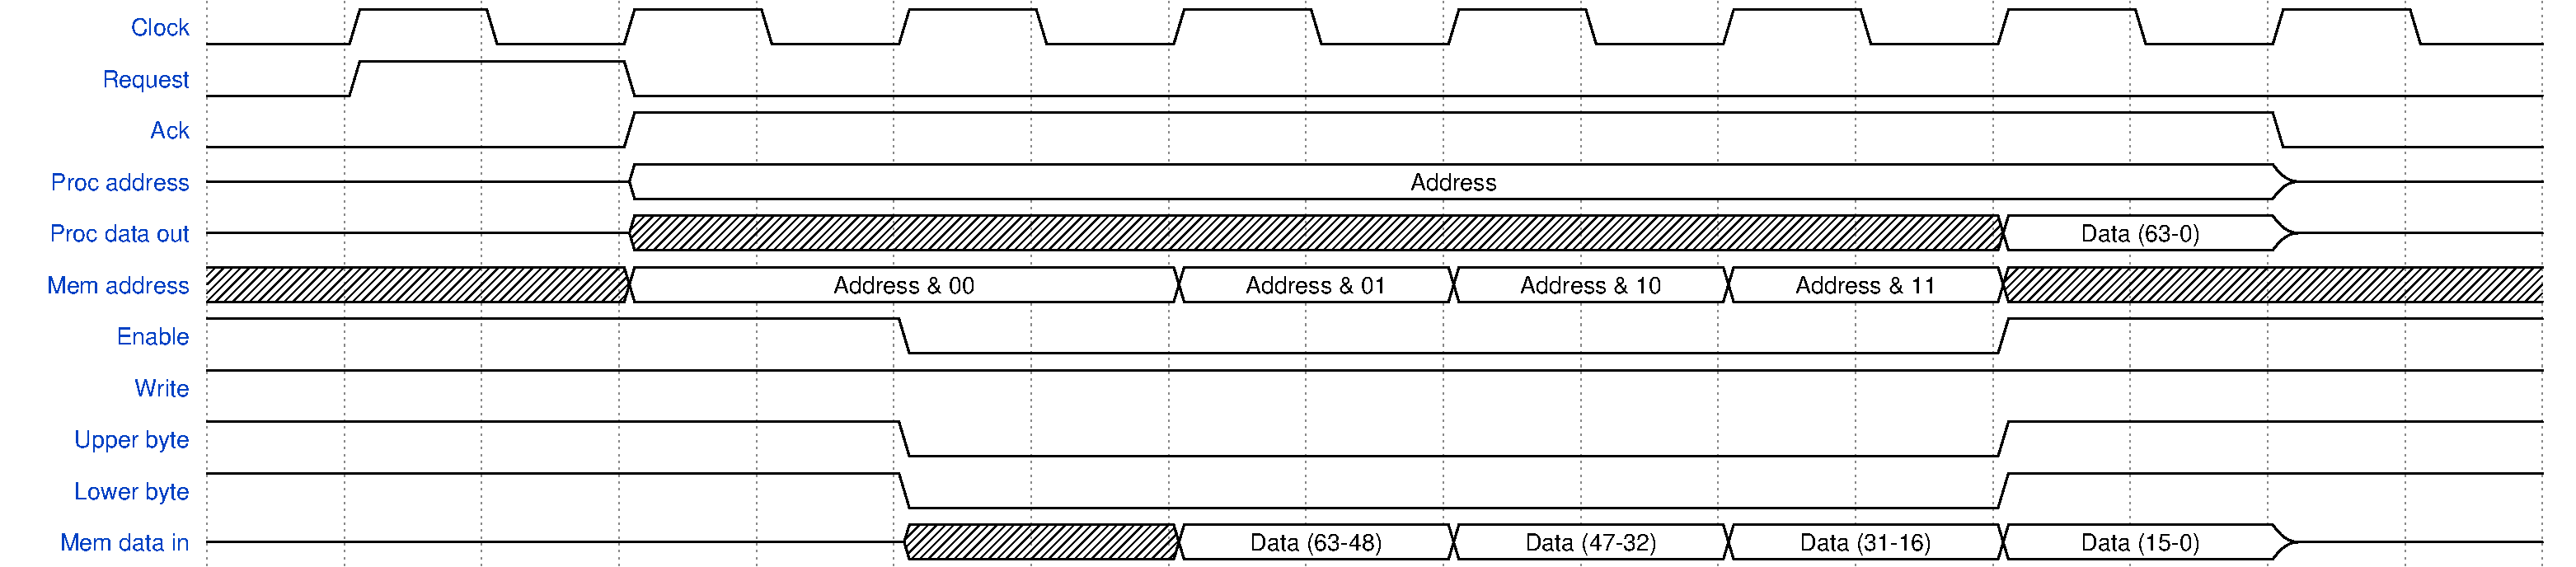
\includegraphics[width=\textwidth]{fpga/fig/timing/data_mem_read.pdf}
  \caption{Data memory read cycle}
  \label{fpga:fig:timing:dmem:read}
\end{figure}

\begin{figure}[H]
  \centering
  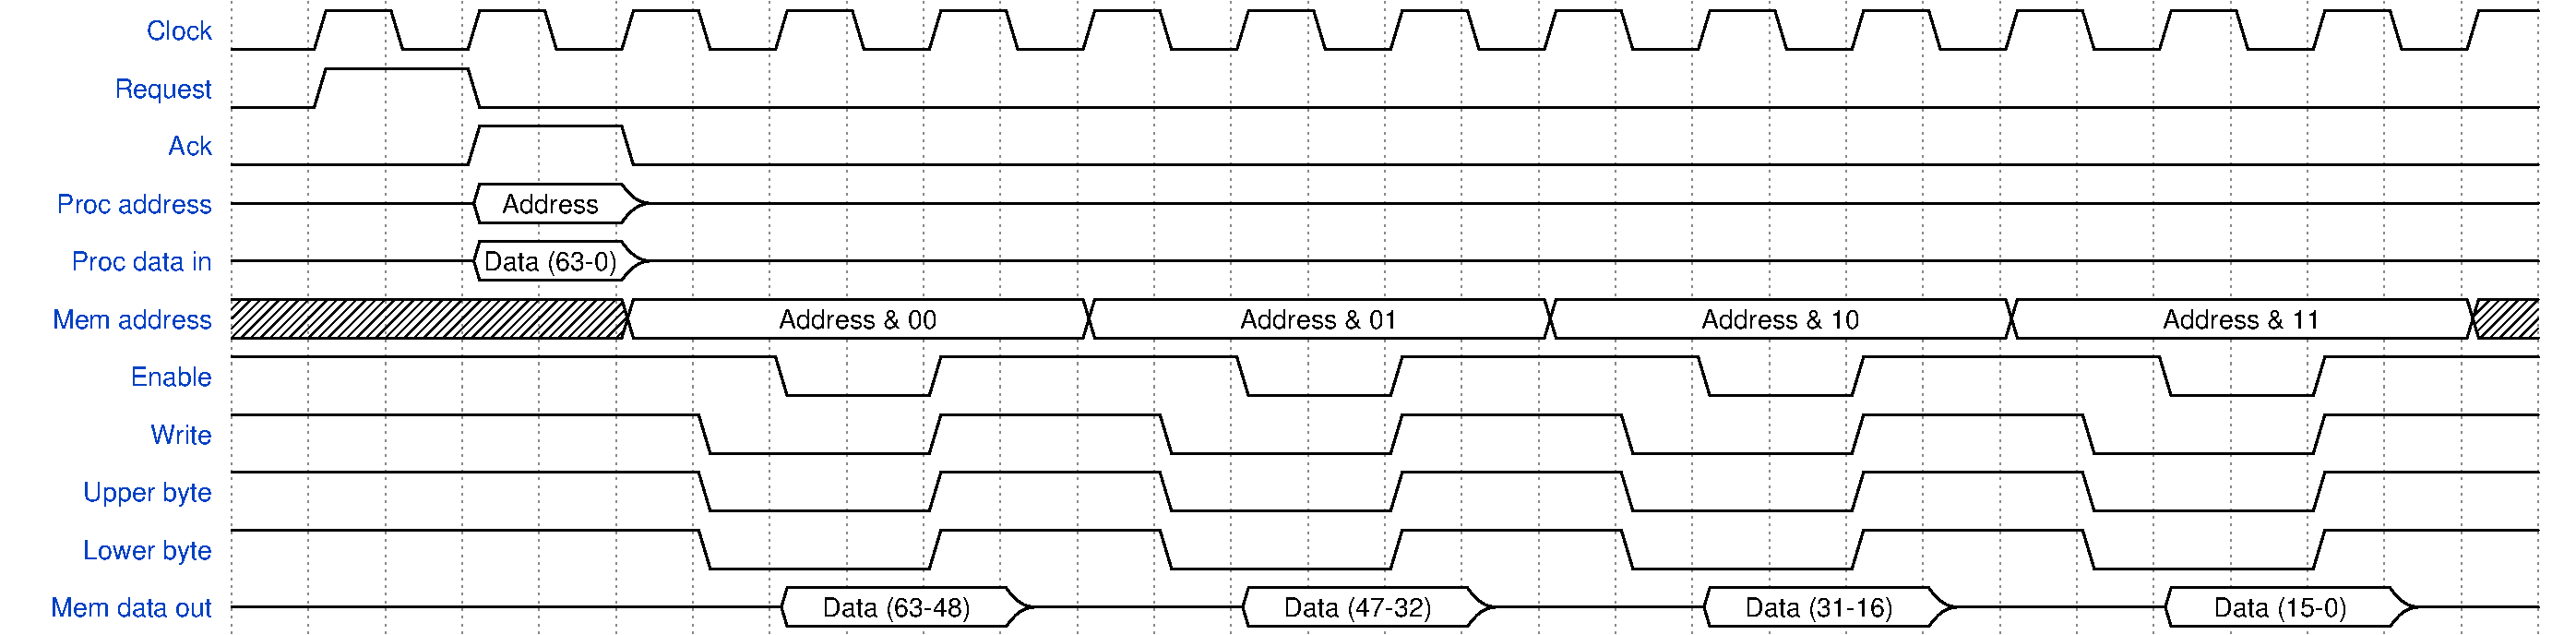
\includegraphics[width=\textwidth]{fpga/fig/timing/data_mem_write.pdf}
  \caption{Data memory write cycle}
  \label{fpga:fig:timing:dmem:write}
\end{figure}

As is immediately apparent in figures \vref{fpga:fig:timing:dmem:read} and \vref{fpga:fig:timing:dmem:write}, the number of cycles required for load and store operations are are 5 and 13 cycles, respectively.
A state machine is implemented in the \emph{data memory controller} to handle interfacing with the external memory chips.
This state machine is responsible for controlling that the different signals are set according to the diagrams.
For more detailed view of the \emph{Data memory controller}, the reader is advised to study the state machine diagram in figure \ref{fpga:fig:mem:data_memory_ctrl_state_machine} and the accompanying data path in figure \ref{fpga:fig:mem:data_memory_ctrl}.

\begin{figure}[H]
  \centering
  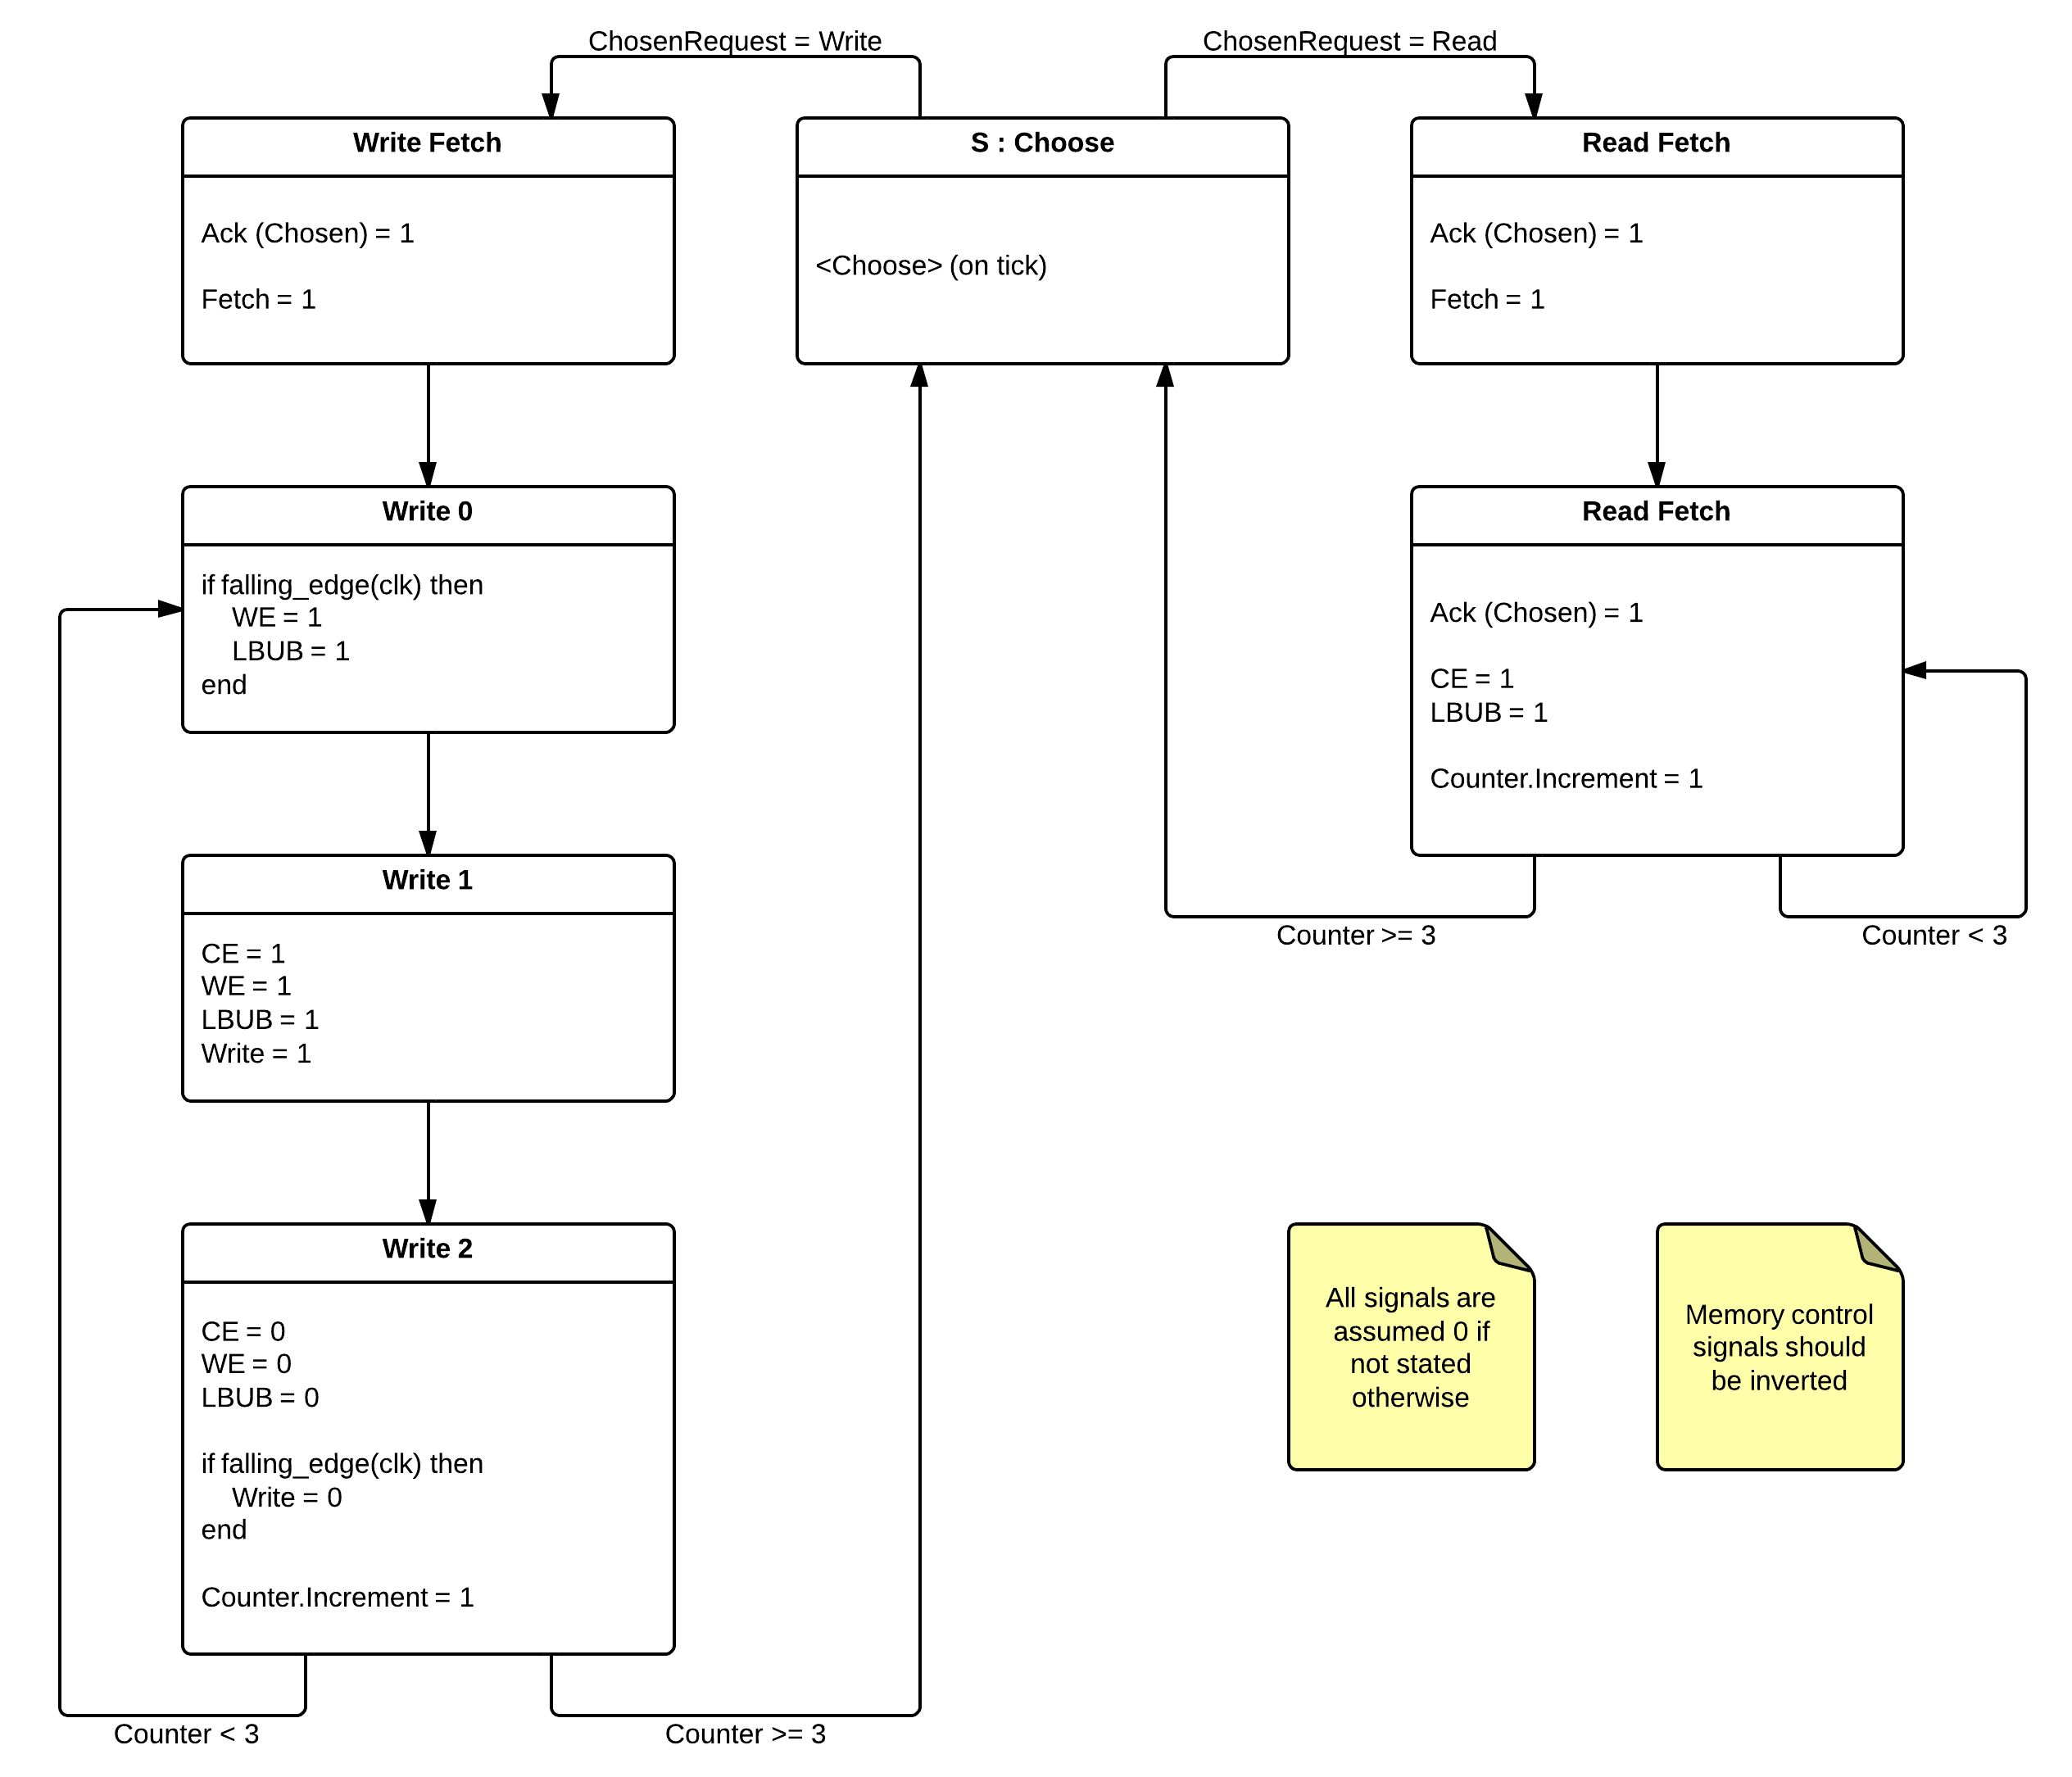
\includegraphics[width=\textwidth]{fpga/fig/memory_ctrl_state_machine.png}
  \caption{Data memory controller state machine}
  \label{fpga:fig:mem:data_memory_ctrl_state_machine}
\end{figure}


\begin{figure}[H]
  \centering
  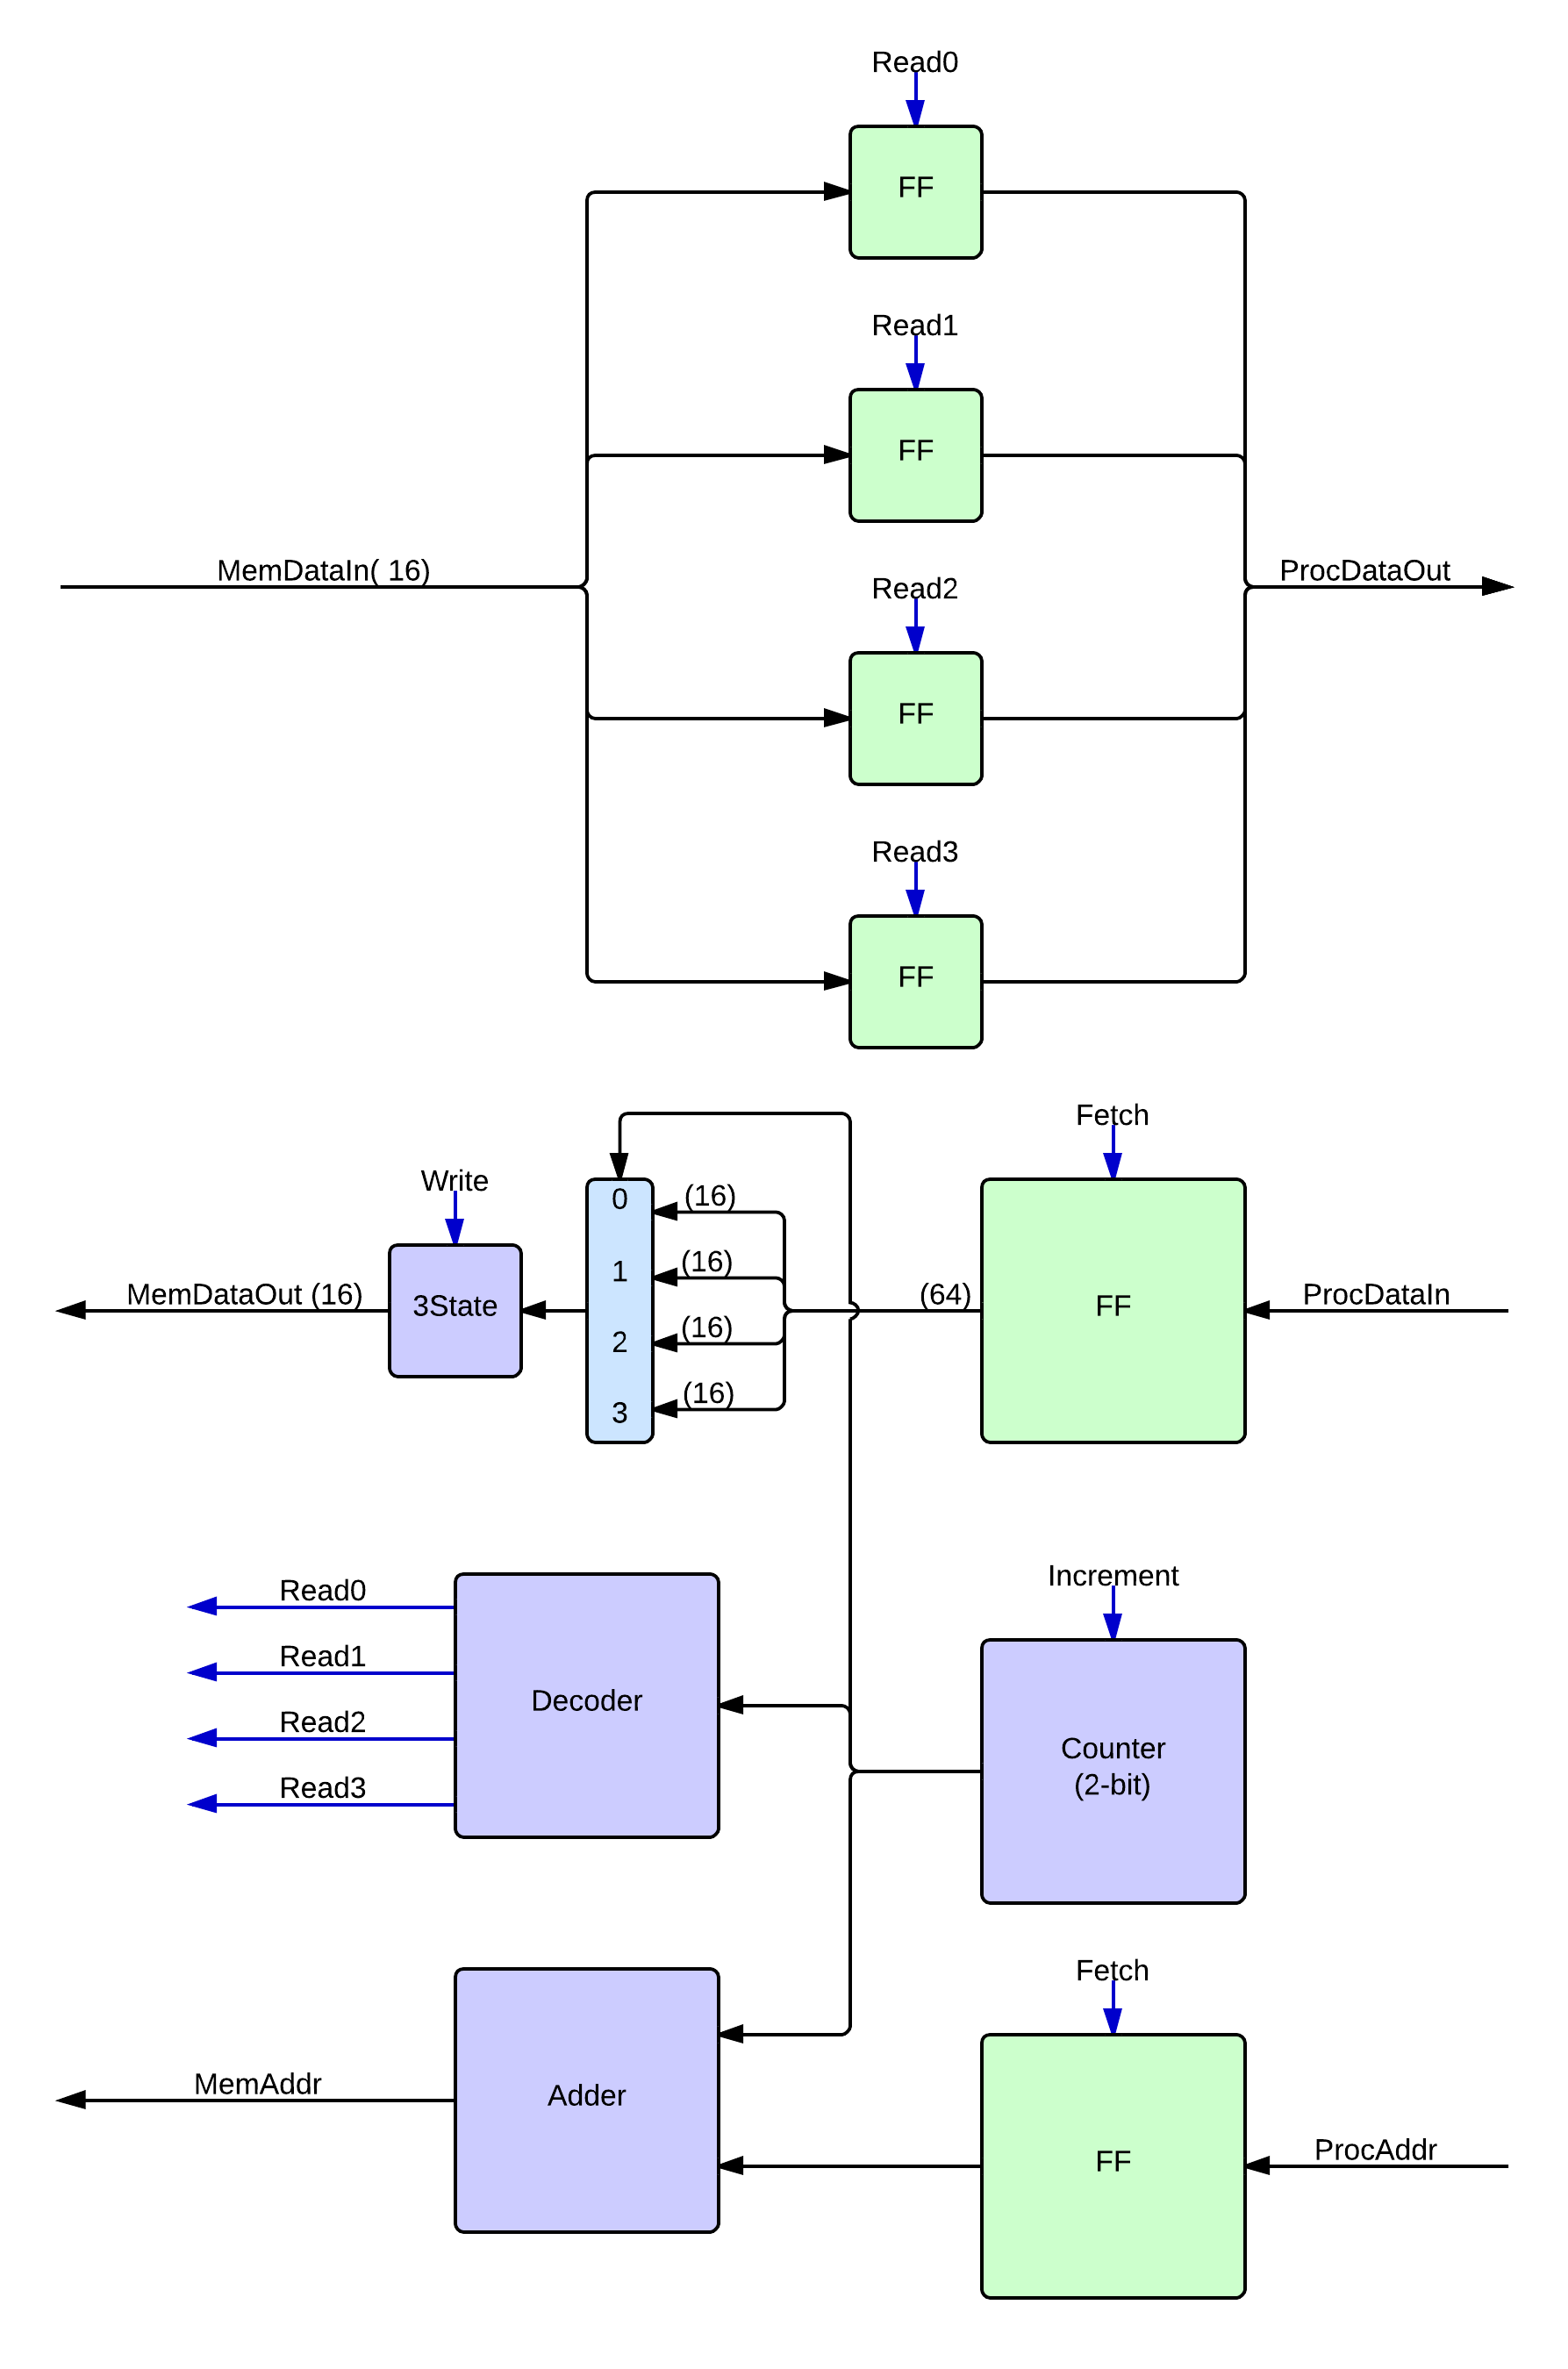
\includegraphics[width=\textwidth]{fpga/fig/memory_ctrl.png}
  \caption{Data memory controller signals mapping}
  \label{fpga:fig:mem:data_memory_ctrl}
\end{figure}

